\subsection{Расчет профиля температур}

Для расчета профиля температур лопатки принимаем расход воздуха $G_в = 0.053 кг/c$, а величину зазора между дефлектором и
внутренней поверхностью лопатки $\delta = 1 мм$.

При расчете профиля температур лопатки при конвективно-пленочно охлаждении будем пользоваться следующей методикой:
\begin{enumerate}
	\item Зададим распределение приведенной скорости по корыту $\lambda_к \left( \overline{x} \right)$ и спинке $\lambda_с \left( \overline{x} \right)$:
		$$
			\lambda_к \left( \overline{x} \right) = 
			\left\{ 
				1 + 
				\left[ 
					\left( 
						\frac{\lambda_1}{\lambda_0}
					\right)^{0.5}
				\right]\overline{x}
			\right\}^{2} \lambda_0, \/\ \overline{x} = \frac{x}{l_к}
		$$
		$$
			\lambda_с \left( \overline{x} \right) = 
			\left\{ 
				1 + 
				\left[ 
					\left( 
						\frac{\lambda_1}{\lambda_0}
					\right)^{4}
				\right]\overline{x}
			\right\}^{0.25}\lambda_0, \/\ \overline{x} = \frac{x}{l_с}
		,$$
		где $l_к$ - длина профиля со стороны корыта, $l_с$ - длина профиля со стороны спинки, $\lambda_0$ - приведенная скорость на входе в лопаточный венец, $\lambda_1$ - приведенная скорость на выходе из лопаточного венца.

	\item Определим критическую скорость звука $a_{кр}$:
		$$
			a_{кр} = \sqrt{
				\frac{2k_г}{k_г + 1} R_г T_г^*
			}
		$$
	\item Определим скорость газа на корыте $v_к$ и на спинке $v_с$:
		$$
			v_к\left( x \right) = \lambda_к \left( \frac{x}{l_к} \right)
		$$
		$$
			v_c\left( x \right) = \lambda_к \left( \frac{x}{l_c} \right)
		$$
	Дальнейший расчет идентичен для спинки и корыта, поэтому скорость газа будем обозначать как $v_г$.
	\item Определим эквивалентную ширину щели:
		$$
			s = N_{отв} \frac{\pi d_{отв}^2}{4} \cdot \frac{1}{l},
		$$
		где $N_{отв}$ - количество отверстий, $d_{отв}$ - диаметр отверстия, $l$ - высота профильной части лопатки.
	\item Определим скорость газа в точке выдува воздуха:
		$$
			v_{г \/\ отв} = v_г\left( x_{отв} \right),
		$$
		где $x_{отв}$ - криволинейная координата отверстия.
	\item Определим статическую температуру газа в точке выдува воздуха:
		$$
			T_{г \/\ отв} = T_г^* - \frac{v_{г \/\ отв}}{2 c_{p \/\ г}}
		$$
	\item Определим статическое давление газа в точке выдува воздуха:
	 	$$
	 		p_{г \/\ отв} = \frac{p_г^*}{
	 			\left( 
	 				\frac{
	 					T_г^*
	 				}{
	 					T_{г \/\ отв}
	 				}
	 			\right)^\frac{k_г}{k_г - 1}
	 		}
	 	$$
	\item Определим статическую плотность газа в точке выдува воздуха:
	 	$$
	 		\rho_{г \/\ отв} = \frac{
	 			p_{г \/\ отв}
	 		}{
	 			R_г \cdot T_{г \/\ отв}
	 		}
	 	$$
	\item Определим скорость истечения воздуха из отверстия:
	 	$$
	 		v_{в \/\ отв} = \phi_{отв} \sqrt{
	 			\frac{2k_в}{k_в - 1}
	 		} R_в \theta \left( x_{отв} \right) 
	 		\left[ 
	 			1 - 
	 			\left( 
	 				\frac{
	 					p_{г \/\ отв}
	 				}{
	 					p_{в0}^*
	 				}
	 			\right)^\frac{k_в - 1}{k_в}
	 		\right],
	 	$$
	 	где $\phi_{отв}$ - коэффициент скорости, $\theta \left( x_{отв} \right)$ - температура воздуха в точке выдува, $p_{в0}^*$ - давление воздуха.
	\item Определим статическую плотность воздуха на выходе из отверстия:
		$$
			\rho_{в \/\ отв} = \frac{
				p_{г \/\ отв}
			}{
				R_в
				\left[
					\theta \left( x_{отв} \right) - \frac{v_{в \/\ отв}^2}{2c_{p \/\ в}}
				\right]
			}
		$$
	\item Определим плотность торможения воздуха на входе в отверстия:
		$$
			\rho_{в \/\ отв}^* = \frac{p_{в0}^*}{R_в \theta \left( x_{отв} \right) }
		$$
	\item Определим параметр вдува:
		$$
			m = \frac{\rho_{в \/\ отв} v_{в \/\ отв}}{\rho_{г \/\ отв} v_{г \/\ отв}}
		$$
	\item Определим число Рейнольдса по ширине щели:
		$$
			Re_s = \frac{
				\rho_{г \/\ отв} v_{г \/\ отв} s
			}{\mu_г\left( T_{г \/\ отв} \right)}
		$$
	\item Определим температурный фактор:
		$$
			\phi = \theta \left( x_{отв} \right) / T_г^*
		$$
	\item Определим эффективность пленки $\theta_{пл}\left( x \right)$:
		$$
			A\left( x \right) = Re_s^{-0.25} m^{-1.3} \phi^{-1.25}
			\left(
				\frac{
					x - x_{отв}
				}{
					s
				}
			\right)
		$$
		$$
			\theta_{пл}\left( x \right) = \left\{
				\begin{array}{@{}ll@{}}
					1.0, & \text{если}\ 0 < A \leq 3 \\
					\left( \frac{A}{3} \right)^{-0.285}, & \text{если} 3 \leq A < 11 \\
					\left( \frac{A}{7.43} \right)^{-0.95}, & \text{если} A \geq 11 \\
				\end{array}\right.
		$$
	\item Определим темперутуру пленки в случае нескольких рядов отверстий:
		$$
			T_{пл}^*\left( x \right) = T_г^* \cdot \prod_{i = 1}^{x_i \leq x}
				\left[
					\left(
						1 - \theta_{пл \/\ i}
					\right)
				\right] + 
				\sum_{i = 1}^{x_i \leq x} \left[
					\theta_{пл \/\ i}T_в^*\left( x_{отв \/\ j} \right)
					\prod_{j = i + 1}^{x_j \leq x} 
					\left(
						1 - \theta_{пл \/\ j}
					\right)
				\right]
		$$
	\item Определим коэффициент теплоотдачи пленки в случае нескольких рядов отверстий:
		$$
			\alpha_{пл}\left( x \right) = \alpha_{г}
			\prod_{i = 1}^{x_i \leq x} \left[
				1 + \frac{
					2m_i
				}{
					\frac{
						x - x_{отв \/\ i}
					}{s_i}
				}
			\right]
		$$
	\item По формуле истечения из сопла определим расход через ряд отверстий:
		$$
			G_отв = s \cdot l \cdot  \mu_{отв} \sqrt{
				\frac{2k_в}{k_в - 1} p_{в0}^*\rho_{в \/\ отв}^* 
				\left(
					\frac{
						p_{г \/\ отв}
					}{
						p_{в0}^*
					}
				\right)^\frac{2}{k_в}
				\left[
					1 - 
					\left(
						\frac{
							p_{г \/\ отв}
						}{
							p_{в0}^*
						}
					\right)^\frac{k_в - 1}{k_в}
				\right]
			}
		$$
	\item В общем случае зависимость расхода воздуха в зазоре от криволинейной координаты имеет вид:
		$$
			G_в \left( x \right) = G_{в0} - \sum_{i = 1}^{x_i \leq x} G_{отв \/\ i}
		$$

В данном расчете суммарный расход на охлаждение сопловых лопаток принимается равным
$G_0 = 45 \cdot 10^{-3} \/\ кг/c$ на лопатку, что при числе лопаток статора, равном 54, равно 4.89\% от суммарного расхода
воздуха.
В результате расчетов получим значения характерных параметров в отверстиях.

Значения характерных параметров в отверстиях корыта представлены в табл. ~\ref{cool2:ps_hole_parameters}.
\begin{longtable}{|c|c|c|c|c|c|c|c|c|}
	\caption{Значения характерных параметров в отверстиях корыта}
	\label{cool2:ps_hole_parameters}
	\hline
	\textbf{№} &
	\textbf{$x, \/\ мм$} & 
	\textbf{$s, \/\ 10^{-3} \/\ мм$} &
	\textbf{$\phi_{отв}$} &
	\textbf{$\mu_{отв}$} &
	\textbf{$m$} & 
	\textbf{$\phi$} & 
	\textbf{$G_{отв}, \/\ 10^{-3} \/\ кг/с$} &
	\textbf{$G_{отв} / G_{в0}$} 
	\\ \hline
	\endhead
	
		1 & 
		4.0 & 
		79.5 &
		0.98 &
		0.98 &
		2.08 &
		0.42 &
		5.25 &
		0.131 
		\\\hline
	
		2 & 
		18.0 & 
		62.8 &
		0.98 &
		0.98 &
		1.87 &
		0.54 &
		3.60 &
		0.090 
		\\\hline
	
		3 & 
		30.0 & 
		98.2 &
		0.98 &
		0.98 &
		1.77 &
		0.63 &
		5.18 &
		0.129 
		\\\hline
	
		4 & 
		37.0 & 
		62.8 &
		0.98 &
		0.98 &
		1.76 &
		0.64 &
		3.25 &
		0.081 
		\\\hline
		
\end{longtable}

Значения характерных параметров в отверстиях спинки представлены в табл. ~\ref{cool2:ps_hole_parameters}.
\begin{longtable}{|c|c|c|c|c|c|c|c|c|}
	\caption{Значения характерных параметров в отверстиях спинки}
	\label{cool2:ss_hole_parameters}
	\hline
	\textbf{№} &
	\textbf{$x, \/\ мм$} & 
	\textbf{$s, \/\ 10^{-3} \/\ мм$} &
	\textbf{$\phi_{отв}$} &
	\textbf{$\mu_{отв}$} &
	\textbf{$m$} & 
	\textbf{$\phi$} & 
	\textbf{$G_{отв}, \/\ 10^{-3} \/\ кг/с$} &
	\textbf{$G_{отв} / G_{в0}$} 
	\\ \hline
	\endhead
	
		1 & 
		7.0 & 
		79.5 &
		0.98 &
		0.98 &
		2.03 &
		0.44 &
		5.12 &
		0.128 
		\\\hline
	
		2 & 
		22.0 & 
		24.5 &
		0.98 &
		0.98 &
		1.87 &
		0.54 &
		1.41 &
		0.035 
		\\\hline
	
		3 & 
		27.0 & 
		24.5 &
		0.98 &
		0.98 &
		1.84 &
		0.57 &
		1.37 &
		0.034 
		\\\hline
	
		4 & 
		32.0 & 
		40.2 &
		0.98 &
		0.98 &
		1.80 &
		0.60 &
		2.18 &
		0.055 
		\\\hline
	
		5 & 
		38.0 & 
		48.1 &
		0.98 &
		0.98 &
		1.76 &
		0.64 &
		2.52 &
		0.063 
		\\\hline
	
		6 & 
		43.0 & 
		79.5 &
		0.98 &
		0.98 &
		1.75 &
		0.66 &
		4.07 &
		0.102 
		\\\hline
		
\end{longtable}


	\item Определим коэффициент теплоотдачи от газа на входной кромке лопатки $\alpha_{г.вх.кр.}$:
		$$
			\alpha_{г.вх.кр.} = 0.74 \frac{
				\lambda_г
			}{
				d_{вх.кр.}
			}\sqrt{
				\frac{
					\rho_г \cdot c_a \cdot d_{вх.кр.}
				}{
					\mu_г
				}
			} =
		$$
		$$
			= 0.74 \frac{
				92.9 \cdot 10^{-3}
			}{
				2.20 \cdot 10^{-3}
			}\sqrt{
				\frac{
					4.3 \cdot 
					110.8 \cdot 
					2.20 \cdot 10^{-3}
				}{
					52.1 \cdot 10^{-6}
				}
			} = 4424.3 \/\ Вт/\left( м^2 \cdot К\right)
		$$
	\item Определим коэффициент теплоотдачи на спинке на расстоянии $\frac{1}{3} b_a$ $\alpha_{г.вых.кр.}$:
		$$
			\alpha_{г.вых.кр.} = 1.5 \alpha_г = 
			1.5 \cdot 1110.5 = 1665.8 Вт/\left( м^2 \cdot К\right)
		$$
	\item Определим коэффициент теплоотдачи на остальной выпуклой части (спинке) $\alpha_{г.сп.}$:
		$$
			\alpha_{г.сп.} = 0.6 \alpha_г = 0.6 \cdot 1110.5 = 666.3 Вт/\left( м^2 \cdot К\right)
		$$
	\item Определим коэффициет теплоотдачи на вогнутой части профиля (корыте) $\alpha_{г.кор.}$:
		$$
			\alpha_{г.кор.} = \alpha_г = 1110.5 = 1110.5 Вт/\left( м^2 \cdot К\right)
		$$
	\item Коэффициент теплоотдачи от стенки к охлаждающему воздуху зависит от его температуры и определяется следующим уравнением $\alpha_{в}$:
		$$
			\alpha_{в} = 0.02 \cdot \frac{
				\lambda_{в}
			}{
				2\delta
			} \left( 
				\frac{
					G_в
				}{
					l
				} \cdot \frac{
					1
				}{
					\mu_{в}
				}
			\right)^{0.8}
		$$

	\item Уравнение теплообмена между охлаждающим воздухом и газом имеет вид:
		$$
			\frac{d\theta}{dx} = \frac{
				2
			}{
				G_в C_{p \/\ в}
			} \frac{
				k_x
			}{
				\alpha_г
			} \left( 
				T_{пл}^* - \theta
			\right),
		$$
	где $k_x$ - коэффициент теплопередачи, определяемый уравнением
		$$
			k_x = \frac{1}{
				\frac{1}{
					\alpha_{пл}
				} + 
				\frac{1}{
					\alpha_в
				} + 
				\frac{\Delta}{\lambda_м}
			}
		$$
	Численно решая уравнение теплообмена, поулчим распределение параметров по спинке и корыту.
	Распределение параметров газа по спинке представлено в табл. ~\ref{cool2:ss_gas_parameters}.
		\begin{longtable}{|c|c|c|c|c|c|}
		\caption{Распределение параметров газа по спинке}
		\label{cool2:ss_gas_parameters}
		\hline
		\textbf{№} &
		\textbf{$x, \/\ м$} & 
		\textbf{$\alpha_{пл} \/\ Вт/\left(м^2 \cdot К\right)$} & 
		\textbf{$\alpha_в \/\ Вт/\left(м^2 \cdot К\right)$} & 
		\textbf{$\theta_x, \/\ К$} & 
		\textbf{$T_{ст.x}, \/\ К$} 
		\\ \hline
		\endhead
		
			1 & 
			0.000 & 
			4424.3 & 
			1372.6 &
			500.0 & 
			1236.3
			\\\hline
		
			2 & 
			2.705 & 
			666.3 & 
			1417.6 &
			566.0 & 
			862.0
			\\\hline
		
			3 & 
			5.352 & 
			666.3 & 
			1444.7 &
			614.1 & 
			890.7
			\\\hline
		
			4 & 
			7.863 & 
			916.0 & 
			1459.0 &
			643.1 & 
			643.1
			\\\hline
		
			5 & 
			10.253 & 
			732.6 & 
			1462.0 &
			649.4 & 
			711.9
			\\\hline
		
			6 & 
			12.539 & 
			705.2 & 
			1468.9 &
			664.9 & 
			767.6
			\\\hline
		
			7 & 
			14.741 & 
			694.1 & 
			1479.0 &
			688.1 & 
			825.6
			\\\hline
		
			8 & 
			16.882 & 
			688.1 & 
			1489.2 &
			715.0 & 
			866.4
			\\\hline
		
			9 & 
			18.986 & 
			684.3 & 
			1498.5 &
			743.0 & 
			899.4
			\\\hline
		
			10 & 
			21.078 & 
			681.6 & 
			1507.2 &
			771.3 & 
			928.2
			\\\hline
		
			11 & 
			23.184 & 
			732.3 & 
			1511.6 &
			786.3 & 
			835.7
			\\\hline
		
			12 & 
			25.330 & 
			696.8 & 
			1517.0 &
			805.1 & 
			921.1
			\\\hline
		
			13 & 
			27.539 & 
			803.0 & 
			1521.9 &
			824.7 & 
			840.9
			\\\hline
		
			14 & 
			29.834 & 
			705.4 & 
			1525.4 &
			839.1 & 
			931.2
			\\\hline
		
			15 & 
			32.234 & 
			2806.0 & 
			1532.1 &
			863.7 & 
			863.7
			\\\hline
		
			16 & 
			34.757 & 
			1807.5 & 
			1535.4 &
			874.8 & 
			948.1
			\\\hline
		
			17 & 
			37.417 & 
			1754.0 & 
			1545.6 &
			911.1 & 
			1035.4
			\\\hline
		
			18 & 
			40.227 & 
			1863.9 & 
			1549.4 &
			925.4 & 
			958.8
			\\\hline
		
			19 & 
			43.198 & 
			4267.9 & 
			1556.3 &
			951.4 & 
			951.4
			\\\hline
		
			20 & 
			46.339 & 
			1890.8 & 
			1558.3 &
			957.7 & 
			975.3
			\\\hline
		
		\end{longtable}

	Распределение параметров газа по корыту представлено в табл. ~\ref{cool2:ps_gas_parameters}.
		\begin{longtable}{|c|c|c|c|c|c|}
		\caption{Распределение параметров газа по корыту}
		\caption{cool2:ps_gas_parameters}
		\hline
		\textbf{№} &
		\textbf{$x, \/\ 10^{-3} м$} & 
		\textbf{$\alpha_{пл} \/\ Вт/\left(м^2 \cdot К\right)$} & 
		\textbf{$\alpha_в \/\ Вт/\left(м^2 \cdot К\right)$} & 
		\textbf{$\theta_x, \/\ К$} & 
		\textbf{$T_{ст.x}, \/\ К$} 
		\\ \hline
		\endhead
		
			1 & 
			0.000 & 
			4424.3 & 
			1372.6 &
			500.0 & 
			1236.3  
			\\\hline
		
			2 & 
			2.577 & 
			1110.5 & 
			1424.7 &
			578.0 & 
			974.8  
			\\\hline
		
			3 & 
			5.198 & 
			1417.0 & 
			1444.2 &
			613.2 & 
			613.2  
			\\\hline
		
			4 & 
			7.731 & 
			1208.9 & 
			1450.8 &
			626.4 & 
			724.9  
			\\\hline
		
			5 & 
			10.179 & 
			1169.9 & 
			1463.9 &
			653.5 & 
			818.5  
			\\\hline
		
			6 & 
			12.550 & 
			1153.5 & 
			1480.5 &
			691.5 & 
			890.2  
			\\\hline
		
			7 & 
			14.848 & 
			1144.4 & 
			1495.0 &
			732.5 & 
			940.2  
			\\\hline
		
			8 & 
			17.081 & 
			1138.6 & 
			1507.7 &
			772.9 & 
			979.8  
			\\\hline
		
			9 & 
			19.256 & 
			1346.4 & 
			1512.6 &
			789.4 & 
			797.3  
			\\\hline
		
			10 & 
			21.380 & 
			1210.1 & 
			1515.3 &
			798.8 & 
			856.7  
			\\\hline
		
			11 & 
			23.463 & 
			1177.9 & 
			1519.9 &
			817.0 & 
			916.0  
			\\\hline
		
			12 & 
			25.514 & 
			1162.8 & 
			1526.5 &
			843.3 & 
			964.8  
			\\\hline
		
			13 & 
			27.541 & 
			1153.8 & 
			1534.8 &
			872.7 & 
			1002.0  
			\\\hline
		
			14 & 
			29.555 & 
			1147.7 & 
			1543.4 &
			902.8 & 
			1033.2  
			\\\hline
		
			15 & 
			31.566 & 
			1396.6 & 
			1545.3 &
			910.0 & 
			910.0  
			\\\hline
		
			16 & 
			33.583 & 
			1250.2 & 
			1546.2 &
			913.3 & 
			932.9  
			\\\hline
		
			17 & 
			35.616 & 
			1207.3 & 
			1549.2 &
			924.8 & 
			956.3  
			\\\hline
		
			18 & 
			37.676 & 
			1574.0 & 
			1551.9 &
			934.8 & 
			934.8  
			\\\hline
		
			19 & 
			39.772 & 
			1266.7 & 
			1553.0 &
			939.2 & 
			950.4  
			\\\hline
		
			20 & 
			41.912 & 
			1216.6 & 
			1557.3 &
			954.5 & 
			974.8  
			\\\hline
			
		\end{longtable}

\end{enumerate}

Распределение температур газа, воздуха и металла по профилю лопатки показано на рис. ~\ref{img:cool_gas_parameters_front}.
\begin{figure}[H]
    \centering
	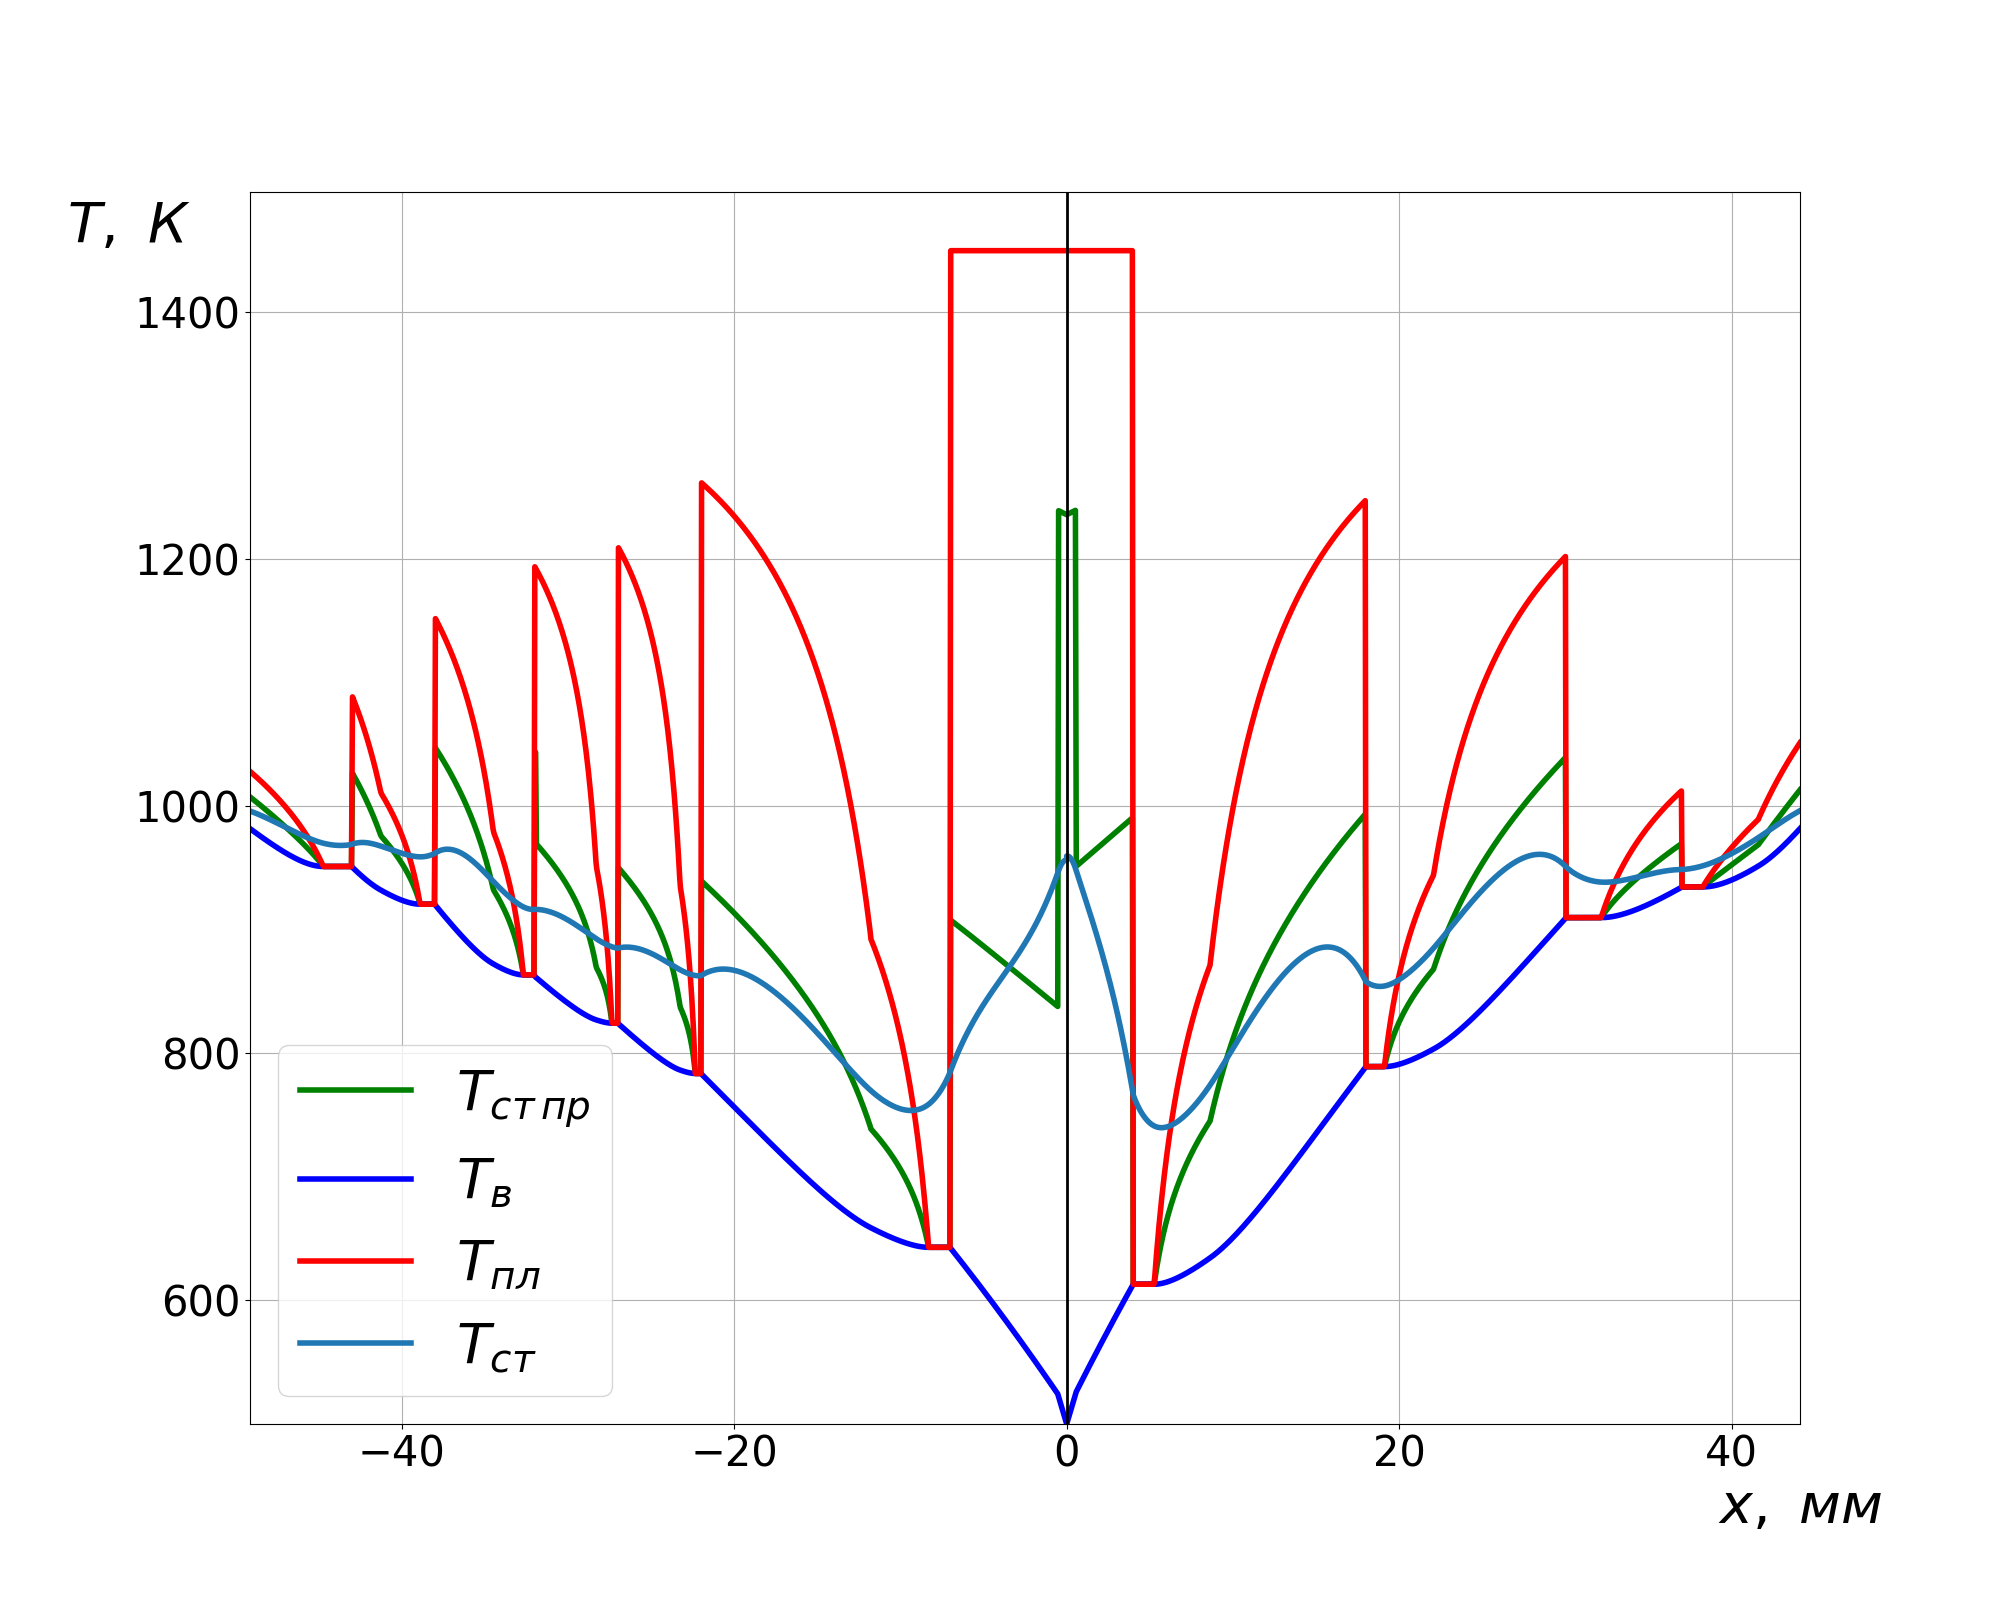
\includegraphics[scale=0.8]{cooling_2_t}
	\caption{Распределение температур газа, воздуха и металла}
	\label{img:cool_gas_parameters_front}
\end{figure}

Также был проанализирован вариант без выдува воздуха в лобовой точке (рис. ~\ref{img:cool_gas_parameters_no_front}).
Однако отсутствие выдува в лобовой точке приводит к сильному перегреву с возможным прогарание профиля лопатки.
\begin{figure}[H]
    \centering
	\includegraphics[scale=0.8]{cooling_2_t_hot}
	\caption{Распределение температур газа, воздуха и металла (без выдува в лобовой кромке)}
	\label{img:cool_gas_parameters_no_front}
\end{figure}

Таким образом, из расчета следует, что ни в одной точке температура материала лопатки не превышает 1100 К (максимальная температура
равна 1081 К), что в случае равномерного поля температур перед сопловыми лопатками обеспечивает достаточную прочность лопаток [1].
Однако основной причиной выхода из строя сопловых лопаток является не температурная деформация, а коррозия.
Для защиты от воздействия агрессивной среды сопловые лопатки покрываются защитным керамическим покрытием на основе
$Zr0_2$ с металлической подложкой на основе $Ni-Cr-Al-Y$. Такой состав покрытия обеспечивает его хорошую адгезию к
основному материалу лопатки и предотвращает его от растрескивания под действием термоциклических нагрузок.
Побочным эффектом применения данного покрытия является снижение температуры основного материала лопатки на 50-60 К
вследствие крайне низкой теплопроводности керамического слоя покрытия.
